\documentclass[a4paper]{report}
\usepackage{amsmath} 
\usepackage{graphicx}

\title{DDPG + HER in FetchPush-v1 Gym Environment with Python3 and Tensorflow 2.0}
\author{Simone De Angelis 1760464\\ Veronica Romano 1580844}
\date{\today}


\begin{document}

\maketitle

\chapter{Introduction and Work Purposes}
Reinforcement Learning is learning what to do and how to map situations to actions. The end result is to maximize the numerical reward. The learner is not told which action to take, but instead must discover which action will yield the maximum reward. As illustrated in Figure \ref{Fig: scheme}, an agent, which is who have to reach a goal, stars from a state s\_t and through actions a\_t, manipulates the environment. From this it takes a reward r\_t+1, if goes more close to the goal and it's intended to encourage good agent behavior, and discovers the next state s\_t+1. These two are the reward and the state that permits the agent to re-implement the cycle. 

\begin{figure}[h!]
\centering
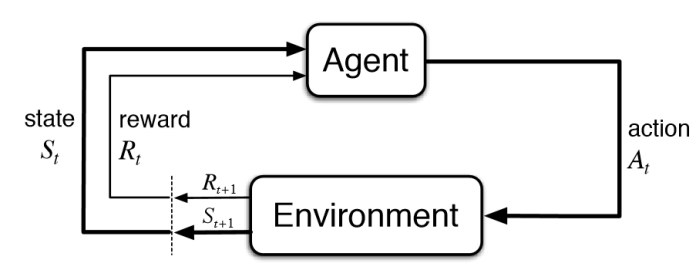
\includegraphics[scale=0.5]{reinforcement.jpg}
\caption{\label{Fig: scheme} Formulation of a basic Reinforcement Learning project.}
\end{figure}

This proceeds until the goal is reached. 

%Reinforcement Learning also differs from the other machine learning techniques. In fact in supervised learning there is a "supervisor" which has the knowledge of the environment and shares it with the agent to complete the task. while in reinforcement learning is the agent that learns from its own experience. Moreover there is a reward function which acts as a feedback to the agent. With respect to unsupervised learning where there is no mapping from input to output, in reinforcement learning the mapping is present. 
%This type of learning is usually modeled through Markov Decision Process. If the environment is non-deterministic we need a transition model $P(s'|s,a)$ and the utility function is the sum of the received rewards.

In few words, an \textit{agent} has a set of \textit{action space} which it can perform in a given \textit{environment} for which it gets \textit{rewarded} if that action meets some criteria. The agent ought to take actions to maximize this reward.
This is the basic principle of reinforcement learning. In particular reinforcement learnin is a field of artificial intelligence that has several applications in the robotics field, which is the field of this project. 
OpenAI gym is a open source tool that allows us to work with algorithm for reinforcement. Previously there aren't many standard environment that could be used to the developed of these algorithms. In fact the rise of Gym, reinforcement learning becomes more practical and implementable with respect to the traditional machine learning methods. Gym is available on the corresponding GitHub repository. On the other hand there is also MuJoCo (Multi-Joint dynamics with Contact). This is a physical engine for detailed, efficient rigid body simulations with contacts. It has a dynamic library with C/C++ API. mujoco\-py allows using MuJoCo from Python 3. It includes an XML parser, model compiler, simulator, and interactive OpenGL visualizer. To use it a specific license is needed; we use this for visualizing and using our environment, and to provide a graphical visualization of the results reached. MuJoCo is also customizable, so the environment can be modified by changing its XML code. This permits also to create new environments for implementing new tasks. However the best part is that MuJoCo provides the physical interactivity (like calculation of contact forces) which helps an engineer or researcher to test their model rigorously before moving to production.
\\


This work consists in implementing the FetchPush-v1 environment provided by Gym OpenAI (using MuJoCo as physical simulator), and using a specific algorithm, which in our specific case is DDPG+HER, experimenting on this environment. Also a specific framework will be assigned for the implementing the code. All the result reached will be illustrated in Chapter \ref{exp}. While in the following sections we will exploit in details the algorithm used for our task, the environment, and the implementation framework.


\chapter{Implementation Assignment}
To implement this work a specific framework has been assigned. We have used Python3 and TensorFlow 2.0. In particular we used TensoFlow for building the neural networks for our actor and critic.


\section{DDPG + HER Algorithm}
Deep Deterministic Policy Gradient (DDPG) is an off-policy algorithm for Reinforcement Learning which concurrently learns a Q-function and a policy. It uses off-policy data and the Bellman equation to learn the Q-function, and uses the Q-function to learn the policy. DDPG, being an actor-critic technique, consists of two models: Actor and Critic. The Actor is a policy network that takes the state as input and outputs the exact action (continuous), instead of a probability distribution over actions. The Critic is a Q-value network that takes state and action as input and outputs the Q-value. DDPG is used in the continuous action setting and the word "Deterministic" in DDPG refers to the fact that the actor computes the action directly instead of a probability distribution over actions. This approach is closely connected to Q-learning, and is motivated the same way: if you know the optimal action-value function $Q^*(s,a)$, then in any given state, the optimal action $a^*(s)$ can be found by solving:

\begin{equation}
a^*(s) = argmax_a Q^*(s, a)
\end{equation} 

DDPG put together the learning of an approximator $Q^*(s, a)$ and the learning of an approximator $a^*(s)$, and it does this in a way which is specifically for continuous action spaces. This refers to the way in which the $\max$ over actions is computed in $\max_a Q^*(s, a)$. When there are a finite number of discrete actions, the max poses no problem, because we can just compute the Q-values for each action separately and directly compare them. However, when the action space is continuous, we can't exhaustively evaluate the space, and solving the optimization problem is highly non-trivial. Because the action space is continuous, the function $Q^*(s,a)$ is presumed to be differentiable with respect to the action argument. This allows us to set up an efficient, gradient-based learning rule for a policy $\mu(s)$ which exploits that fact. Then, instead of running an expensive optimization subroutine each time we wish to compute $\max_a Q(s,a)$, we can approximate it with $\max_a Q(s,a) \approx Q(s,\mu(s))$.

 


\section{Gym Environment}
The release provided by OpenAI Gym, contains four environments using the Fetch research platform. These environments use the MuJoCo physics simulator. Our environment is, as previously mentioned, FetchPush-v1 (Figure \ref{Fig: fetchpush}). Fetch goal is to move a box by pushing it until it reaches a desired goal position. This tasks has the concept of a "goal". By default it uses a sparse reward of -1 if the desired goal was not yet achieved and 0 if it was achieved (within some tolerance). This because the sparse rewards are more realistic in robotics applications and the developers encourage their use.

\begin{figure}[h!]
\centering
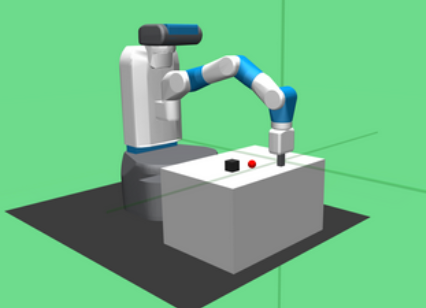
\includegraphics[scale=0.5]{fetchpush.png}
\caption{\label{Fig: fetchpush} FetchPush-v1 Gym environment.}
\end{figure}


\chapter{Experiments and Results \label{exp}}

\end{document}